\section{Теоритические сведения}
Ферромагнитные материалы часто применяются в трансформаторах, дросселях, машинах переменного тока, то есть в устройствах, где
они подвергаются периодическому перемагничиванию,~---
 поэтому изучение магнитных характеристик ферромагнетиков в переменных полях
 представляет большой практический интерес. Основные характеристики
 ферромагнетиков~--- их коэрцитивное поле $H_{C}$, магнитная проницаемость
 $\mu$, рассеиваемая в виде тепла при перемагничивании мощность~--- 
 зависят от частоты перемагничивающего поля. В данной работе кривые гистерезиса ферромагнитных материалов изучаются в поле частоты $ \nu_{0} = 50\;\text{Гц}$ с помощью электронного осциллографа.

 \begin{figure}[ht!]
     \center{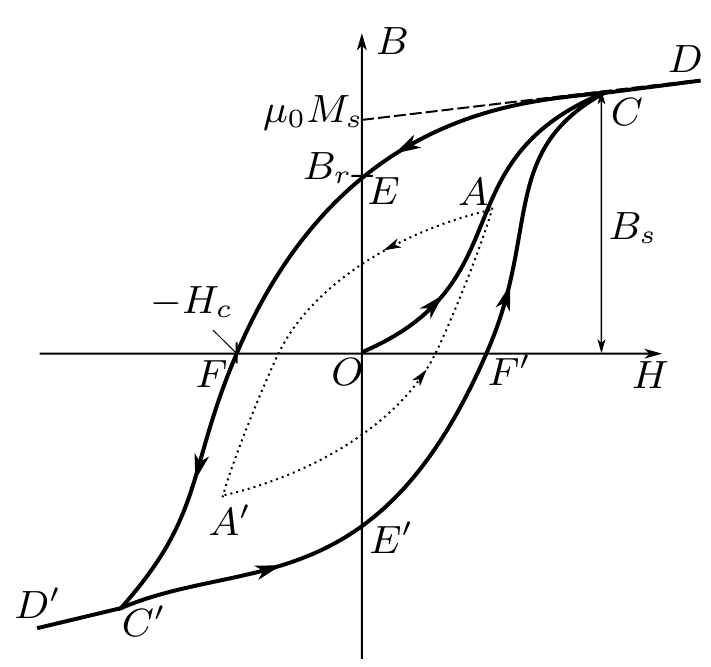
\includegraphics[width=0.5\linewidth]{../img/1.png}}
 \end{figure}
 
 Магнитная индукция $B$ и напряжённость поля $H$ в ферромагнитном материале неоднозначно связаны между собой: индукция зависит
 не только от напряжённости, но и от предыстории образца. Связь между $B$ и $H$ типичного ферромагнетика иллюстрирует рисунок.

Если к ферромагнитному образцу прикладывать переменное внешнее
магнитное поле, то его состояние на плоскости $HB$ будет изменяться
по замкнутой кривой~--- петле гистерезиса. Размер петли определяется
максимальным значением напряжённости $H$ в цикле.
Если амплитуда напряжённости достаточно велика, то образец будет периодически достигать насыщения,
что на рисунке соответствует кривой  CEFC'E'F'C  (предельная петля
гистерезиса). Пересечение предельной петли с вертикальной осью соответствует остаточной индукции $B_{r}$,  пересечение с горизонтальной осью~--- коэрцитивному полю $H_{C}$.
 Крайние точки петель, соответствующие амплитудным значениям $H$.

 Магнитную индукцию $B$ удобно определять с помощью ЭДС, возникающей при изменении магнитного
 потока $\Phi$ в катушке, намотанной на образец. Пусть катушка c $N$ 
  витками плотно охватывает образец сечением $S$, и индукция $B$ в образце
  однородна.
  \[
      |B| = \frac{1}{SN}\int\mathcal{E}dt
  \]
 
  Таким образом, для определения $B$ нужно проинтегрировать сигнал,
  наведённый меняющимся магнитным полем в измерительной катушке,
  намотанной на образец.

  Для интегрирования в работе используется интегрирующая RC-цепочка.
\[
    U_{\text{вых}} = \frac{q}{C} = \frac{1}{C}\int Idt\approx \frac{1}{\tau}\int U_{\text{вх}}dt
\]
$\tau = RC$.

\[
    \frac{U_{\text{вых}}}{U_{\text{вх}}}\approx \frac{1}{\omega_{0}t}
\]
\[
    \tau = RC \gg \frac{1}{\omega_{0}}
\]


